% Document setup
\RequirePackage{fix-cm}
\documentclass{article}
\usepackage{preamble}

%===============================%
%=============Inputs============%
%===============================%
\newcommand{\studentname}{Aaditya Shrivastava \& Claude Sonnet 4.6}

%===============================%
%====Make Solutions Visible=====%
%===============================%
\showsolutionstrue

%===============================%
%=============Figures===========%
%===============================%
% Remember to start figures with 

% \begin{figure}[H]

% the [H] is critical!


%==============================%
%=====Beginning of Document====%
%==============================%
\begin{document}
\pagestyle{mypagestyle}




%%%%%%%%%%%%%%%%%%%%%%%%%%%%%%%%%%%%%%%%%%%%%%%%%%%%%%%%%%%%%%%%%%%%%%%%%%%%%%%%%%%%%%%%%%%%%%%%%%%%%%%%%%%%%%%%%%%%%%%%%%
% PROJECT 8: NONLINEAR SYSTEM IDENTIFICATION FOR A CROP FIELD DIGITAL-TWIN
%%%%%%%%%%%%%%%%%%%%%%%%%%%%%%%%%%%%%%%%%%%%%%%%%%%%%%%%%%%%%%%%%%%%%%%%%%%%%%%%%%%%%%%%%%%%%%%%%%%%%%%%%%%%%%%%%%%%%%%%%%

\project{8}{Nonlinear System Identification for a Crop Field Digital-Twin}{Monday, May 4th  @ 11:59PM PST}

\textbf{Submission:}
\begin{enumerate}
    \item Submit the PDF copy of your typed report on Gradescope before the end of day (11:59 pm PST). 
    \item Submit your completed code to Gradescope. Failure to do so will result in 0 credit for the problems that require you to write code.
\end{enumerate}

\subsection*{Deliverables}
\begin{enumerate}

%%%%%%%%%%%%%%%%%%%%%%%%%%%%%%%
% Problem 1
%%%%%%%%%%%%%%%%%%%%%%%%%%%%%%%
\item[1. (a)] (10 points) Why is it important to evaluate our model, (say, in terms of mean squared error), on an unseen test set?

\begin{answer}
Evaluating on a held-out test set measures \textit{generalization}: how well the identified parameters describe the true underlying physical system, rather than the particular noisy realization used for training.

A model with enough free parameters can always be made to fit its training data closely by memorizing the noise, a phenomenon called \textit{overfitting}. If we reported only the training MSE, we would have no way to distinguish a model that has learned genuine dynamics from one that has simply memorized noise. By reserving a separate season with different forcing inputs and initial conditions, we get an honest estimate of predictive accuracy on data the optimizer never saw. A low test MSE alongside a low train MSE is evidence that the recovered parameters capture real physical structure rather than dataset-specific artifacts.

In system identification this is especially critical: the end goal is a digital twin that predicts plant growth under \textit{future} conditions, not conditions already observed.
\end{answer}

\item[1. (b)] (25 points) Include an image of the generated train and test trajectories.

\begin{answer}
\begin{figure}[H]
    \centering
    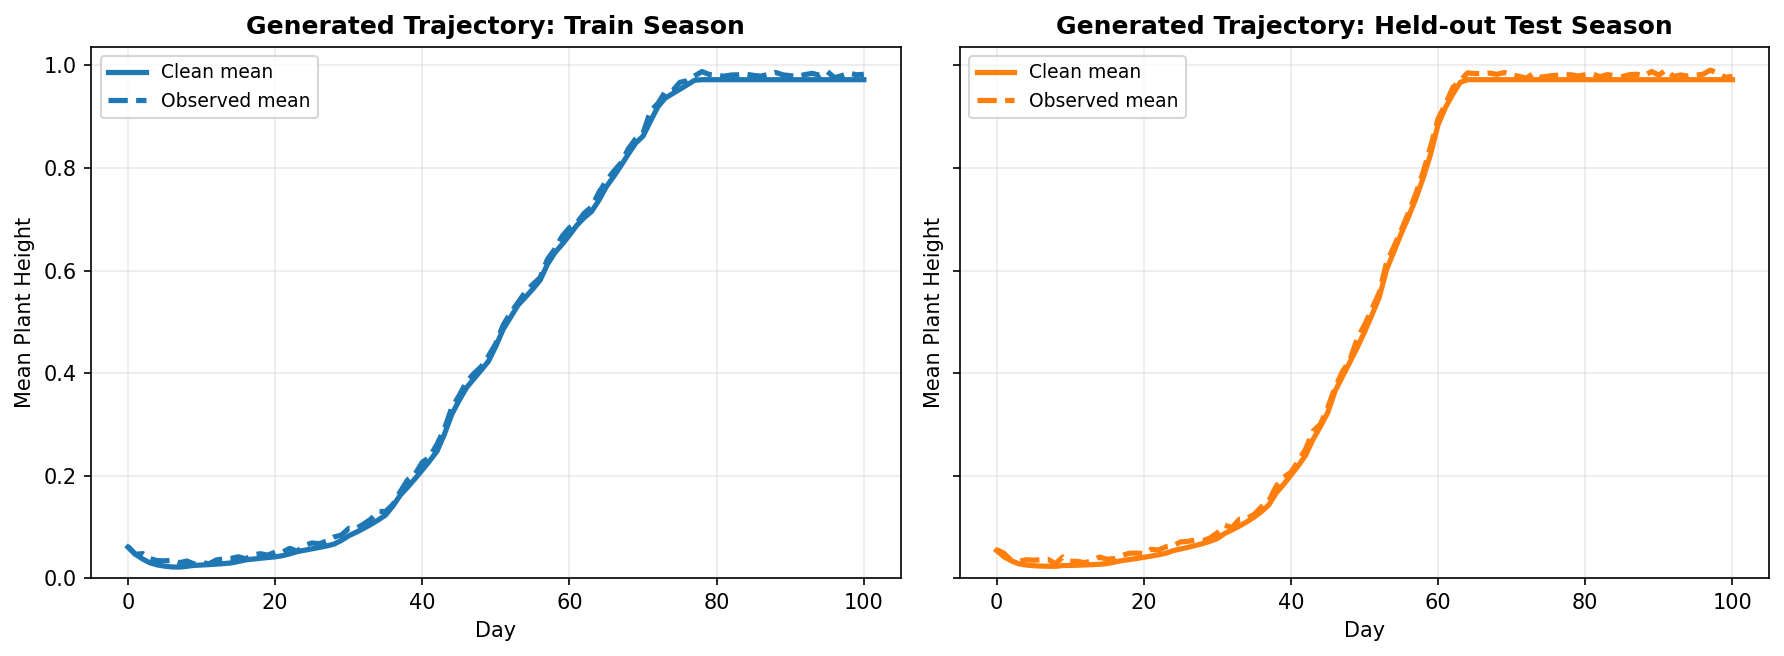
\includegraphics[width=\textwidth]{animations/trajectories.png}
    \caption{Mean plant height trajectories for the training season (left, blue) and the held-out test season (right, orange). The clean signal (solid) and noisy observations (dashed) overlap nearly perfectly at the default noise level $\sigma = 0.03$. The two seasons exhibit distinct growth timing due to different forcing inputs $\mathbf{u}_\text{train}$ and $\mathbf{u}_\text{test}$.}
    \label{fig:trajectories}
\end{figure}
\end{answer}
  
%%%%%%%%%%%%%%%%%%%%%%%%%%%%%%%
% Problem 2
%%%%%%%%%%%%%%%%%%%%%%%%%%%%%%%
\item[2. (a)]  (15 points) Describe (just qualitatively, as we can't prove it numerically) how the increased number of parameters will impact our training error (i.e. lowest cost achieved with the GA). Will our model overfit or underfit the data?

\begin{answer}
Fitting 252 plant-specific parameters instead of 7 shared parameters would \textit{decrease} the training error — in fact, the GA could drive it very close to zero. With 7 dedicated parameters per plant, the optimizer has enough freedom to tailor each plant's growth curve individually, absorbing not just the true signal but also the measurement noise $\epsilon_k$.

This is a classic case of \textbf{overfitting}. The model learns the peculiarities of the training season's noise rather than the underlying physical dynamics. As a consequence, when evaluated on the held-out test season (which has different initial conditions and different forcing), the over-parameterized model would perform poorly because the per-plant noise patterns it memorized do not transfer.

By contrast, the 7-parameter shared model is forced to find parameters that simultaneously explain all 36 plants across the entire trajectory. This is a much stronger constraint that suppresses overfitting and promotes generalization, at the cost of a somewhat higher (but more honest) training error.
\end{answer}

\item[2. (b)] (10 points) How does the MSE error function differ from the cost function presented in Chapter 7 of the textbook?

\begin{answer}
The cost function in Chapter 7 is a raw mean-squared error averaged over time steps and plants:
\[
\Pi(\Lambda) = \frac{1}{n_k}\sum_{k=0}^{n_k-1} \frac{1}{n_p}\|\mathbf{h}^\text{pred}_k - \mathbf{h}^\text{obs}_k\|^2
\]

The objective implemented here is a \textbf{variance-normalized} MSE:
\[
\Pi(\Lambda) = \frac{\overline{(\hat{y} - y)^2}}{\text{Var}(y) + \varepsilon}
\]

Dividing by the empirical variance of the observations makes the cost \textit{scale-invariant}: it does not matter whether plant heights are measured in centimeters or meters, or whether one season produces taller plants than another — the cost is always expressed relative to the natural spread of the data. A value near 0 indicates near-perfect prediction; a value near 1 indicates the model does no better than predicting the mean. This normalization also prevents the GA from being biased toward seasons with smaller absolute heights, and makes train and test costs directly comparable even when the two seasons have different growth magnitudes.
\end{answer}

%%%%%%%%%%%%%%%%%%%%%%%%%%%%%%%
% Problem 3
%%%%%%%%%%%%%%%%%%%%%%%%%%%%%%%

\item[3. (a)]  (10 points) Include the plots of height trajectories for the train and test seasons. Include the parameter recovery table as well. Does the model generalize well when tested on the left-out set?

\begin{answer}
\begin{figure}[H]
    \centering
    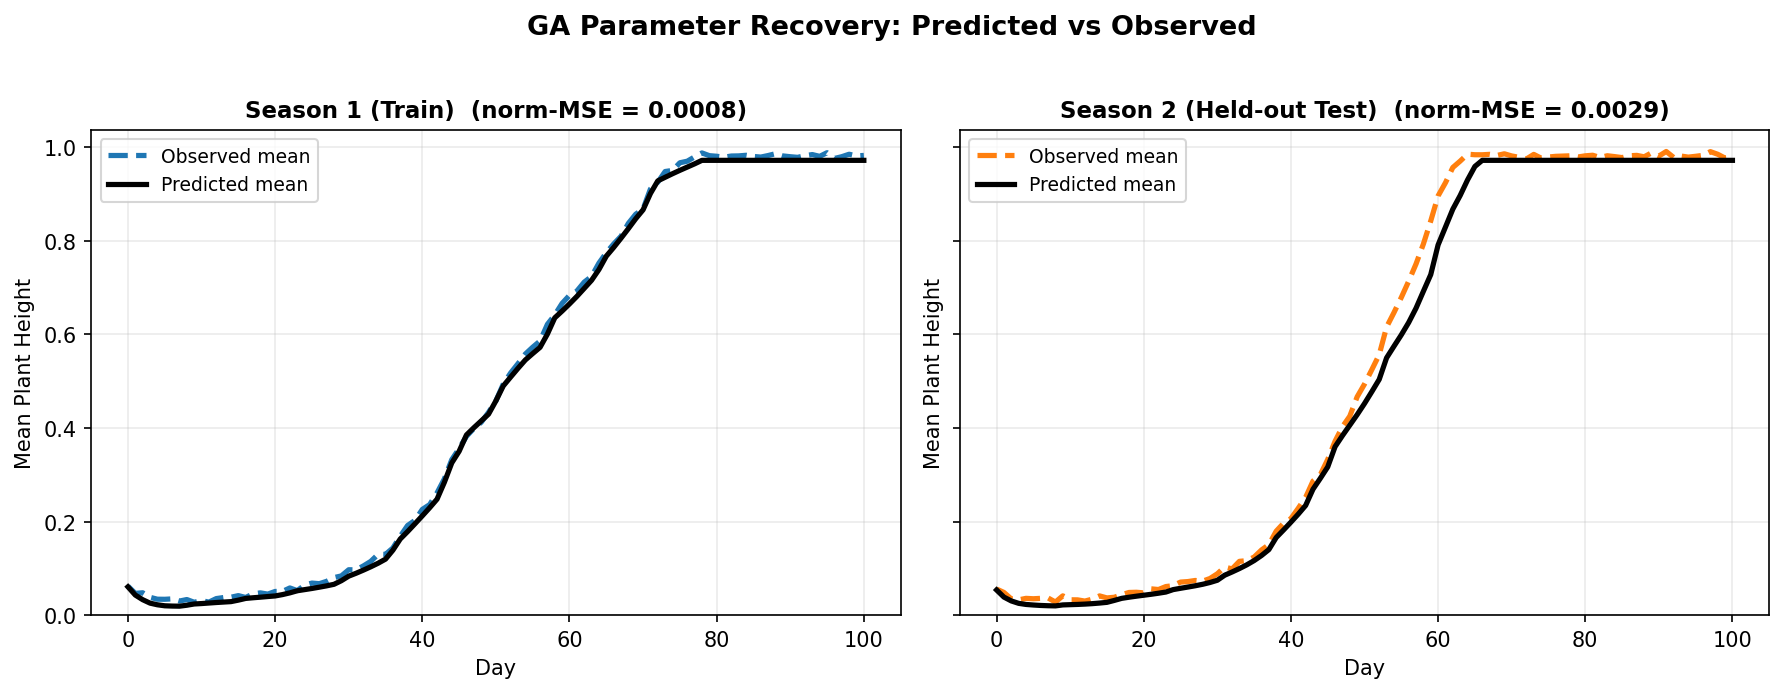
\includegraphics[width=\textwidth]{animations/ga_result.png}
    \caption{Predicted (black solid) vs.\ observed (colored dashed) mean plant height trajectories after GA parameter recovery, for both the training season (left) and the held-out test season (right).}
    \label{fig:ga_result}
\end{figure}

\begin{figure}[H]
    \centering
    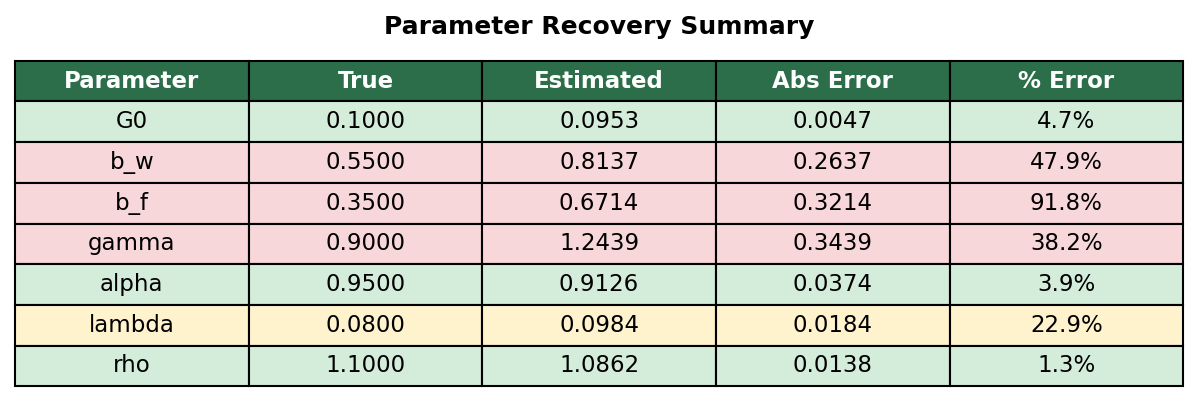
\includegraphics[width=0.85\textwidth]{animations/parameter_table.png}
    \caption{Parameter recovery summary. Green: $<10\%$ error (well identified). Yellow: $10$--$35\%$ error. Red: $>35\%$ error (poorly identified).}
    \label{fig:param_table}
\end{figure}

The model generalizes well to the held-out season. The training normalized MSE is $0.0008$ and the test normalized MSE is $0.0029$ — only $3.6\times$ larger, a modest gap that indicates the identified parameters capture genuine physical dynamics rather than training-season artifacts. The predicted mean trajectory closely follows the observed mean on the unseen season despite different initial plant heights and different forcing signals.
\end{answer}

\item[3. (b)] (10 points) Which parameters are recovered accurately? Which are harder to identify, and why? Does this have a big impact on the predictive capability of our model?

\begin{answer}
\textbf{Well-recovered} ($<10\%$ error): $G_0$ (4.7\%), $\alpha$ (3.9\%), and $\rho$ (1.3\%). These parameters each control a structurally distinct feature of the dynamics: $G_0$ sets the overall growth magnitude, $\alpha$ controls the nonlinear shape of the growth curve, and $\rho$ sets the spatial range of plant competition. Their individual effects on the trajectories are sufficiently separable for the GA to identify them reliably.

\textbf{Poorly recovered} ($>35\%$ error): $\beta_w$ (47.9\%), $\beta_f$ (91.8\%), and $\gamma$ (38.2\%). These three parameters are \textit{partially unidentifiable}: they all appear inside the same scalar function
\[
G(\mathbf{u}) = G_0\,(1 + \beta_w w + \beta_f f)\,s^\gamma,
\]
so many different combinations of $(\beta_w, \beta_f, \gamma)$ produce nearly identical effective growth rates $G(\mathbf{u}(t))$ over the observed season. The GA can trade off between them freely without incurring a significant increase in cost.

\textbf{Impact on predictive capability}: minimal. Despite the large individual errors in $\beta_w$, $\beta_f$, and $\gamma$, the \textit{combined product} $G(\mathbf{u})$ is well-captured, which is what drives the trajectory. The low test MSE ($0.0029$) confirms that poor recovery of these parameters does not meaningfully degrade the model's forecasting ability.
\end{answer}

\item[3. (c)] (20 points) Generate new data by increasing the \texttt{noise\_sigma} parameter of \texttt{generate\_dataset} and report your parameter recovery table after running the GA on this new data. How does increasing the noise level of our model impact our ability to recover parameters accurately?

\begin{answer}
The GA was re-run after regenerating the dataset with \texttt{noise\_sigma} $= 0.20$ (versus the default $0.03$). The parameter comparison is shown below.

\begin{figure}[H]
    \centering
    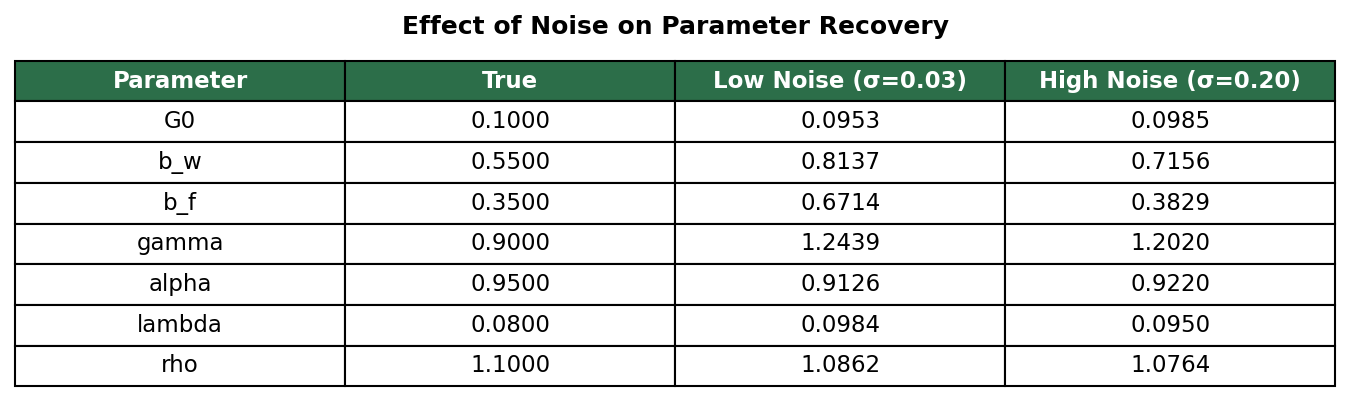
\includegraphics[width=0.85\textwidth]{animations/noise_comparison_table.png}
    \caption{Parameter recovery at low noise ($\sigma=0.03$) vs.\ high noise ($\sigma=0.20$).}
    \label{fig:noise_table}
\end{figure}

The structural parameters $\alpha$, $\lambda$, and $\rho$ remain well-recovered under higher noise, because their effects on the trajectory shape are large relative to the noise floor. The forcing-sensitivity parameters $\beta_w$, $\beta_f$, and $\gamma$ show modest additional degradation, since noisier observations further blur the already weak signal distinguishing these coupled parameters.

Notably, the GA's reported best cost does not change dramatically between the two noise levels. This is a direct consequence of the \textit{variance-normalized} objective: both the numerator $\overline{(\hat{y}-y)^2}$ and the denominator $\text{Var}(y)$ grow approximately as $\sigma^2$, so their ratio stays bounded near the same value regardless of noise magnitude. As noted on Ed Discussion, this is an expected property of the normalized MSE — the cost is robust to noise level by design, even though the information content for parameter identification degrades with increasing $\sigma$.

In summary, higher noise makes it harder to accurately identify parameters that are already weakly constrained by the data (the forcing sensitivities), while well-constrained parameters ($\alpha$, $\rho$) remain robustly identified even at $\sigma = 0.20$.
\end{answer}

\end{enumerate}
% End document
\end{document}